\documentclass[11pt]{article}

\usepackage{graphicx}
\usepackage{mathtools}
\usepackage{listings}
\usepackage{color}
\definecolor{dkgreen}{rgb}{0,0.6,0}
\definecolor{gray}{rgb}{0.5,0.5,0.5}
\definecolor{mauve}{rgb}{0.58,0,0.82}
\lstset{
  language=Java,
  aboveskip=1mm,
  belowskip=1mm,
  showstringspaces=false,
  columns=flexible,
  basicstyle={\small\ttfamily},
  numbers=none,
  numberstyle=\tiny\color{gray},
  keywordstyle=\color{blue},
  commentstyle=\color{dkgreen},
  stringstyle=\color{mauve},
  breaklines=true,
  breakatwhitespace=true,
  tabsize=3
}

\begin{document}
\thispagestyle{empty}

\begin{center}

 \textsc{\Huge Inverse Kinematics}\\

\vspace{-3.5cm} \hspace{-8.5cm}{
\begin{minipage}[]{\linewidth}% to keep image and caption on one page
\center 
\includegraphics[scale=0.3]{/home/alvaro-ferran/Documentos/Frikeo/Hormiguero/M1R0/doc/Latex/bqlogo.png}
\end{minipage}
\hspace{5.5cm}Alvaro Ferr\'an
}

\end{center}

\vspace{2cm} 
\bigskip \flushleft

This document's purpose is to explain how to find the arm's angles when given a position for the end-effector, calculating them geometrically.\\

\begin{minipage}[]{\linewidth}% to keep image and caption on one page
\center 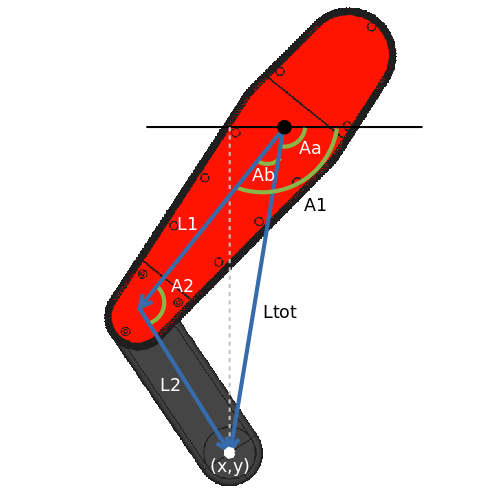
\includegraphics[height=8cm]{/home/alvaro-ferran/Documentos/Frikeo/Hormiguero/M1R0/doc/Latex/Diagrama1.png}
\end{minipage}
\\[0.5cm]
In order to get to position (x,y) we need to find the angles A1 and A2 to which each motor has to move. \\We will start by dividing A1 into two smaller angles: Aa and Ab.
We calculate Aa using the Pythagorean Theorem:

\center $Ltot=\sqrt{x^2+y^2}$
\center $Aa=Acos(\dfrac{x}{Ltot})$

\bigskip 
\flushleft
In order to find Ab, we will use the Law of Cosines:

\center $L2^2=Ltot^2+L1^2-2\cdot Ltot\cdot L1\cdot cos(Ab)$
\center $\rightarrow Ab= Acos(\dfrac{Ltot^2+L1^2-L2^2}{2\cdot Ltot\cdot L1} )$

\flushleft
\bigskip
Thus, 
\center $A1=Aa+Ab$

\newpage 
\thispagestyle{empty}
\flushleft
To find A2 we simply follow the Law of Cosines once more:

\center $Ltot^2=L2^2+L1^2-2\cdot L2\cdot L1\cdot cos(A2)$
\center $\rightarrow A2= Acos(\dfrac{L2^2+L1^2-Ltot^2}{2\cdot L2\cdot L1} )$

\vspace{2.5cm}
\begin{minipage}{\linewidth}%to ensure it stays in the same page

Finally, we implement this algorithm in Java for our Android app:
	\begin{lstlisting}	
 
double[] inverseKinematics(double x, double y) {
	double[] a={0,0};

	double L1=300;
	double L2=200;

	double Ltot=Math.sqrt( Math.pow(x,2) + Math.pow(y,2) );
	double Aa= Math.acos(x/Ltot);
	double Ab= Math.acos( ( Math.pow(Ltot,2) + Math.pow(L1,2) - Math.pow(L2,2) ) / (2*Ltot*L1) );
	double A1=Aa+Ab;
	double A2= Math.acos((Math.pow(L2, 2) + Math.pow(L1, 2) - Math.pow(Ltot, 2)) / (2 * L2 * L1));

	a[0]=A1;
	a[1]=A2;

	return a;
}


\end{lstlisting}
\bigskip
Which may then be called:
\begin{lstlisting}	
double[] angles=inverseKinematics(x,y);
\end{lstlisting}
\end{minipage}

\end{document}
